\section{My view}

\begin{frame}{Starting Point}
  \centering
    \color{Pink} Transfer Learning for DNN Applications for Constitutive Modeling 
\end{frame}

\begin{frame}{My View on Current ML Surrogate Models}
\begin{minipage}{0.45\textwidth}
  \begin{block}{\color{White} Problems}<1>
    \begin{itemize}
      \item <1> Need of abundant data
      \item <1> Problem specific applications 
      \item <1> Single parameter considerations
    \end{itemize}
  \end{block} 
\end{minipage}%
\hspace{1cm}
\end{frame}

\begin{frame}{Holistic Problem}
\centering
\includegraphics[width=0.6\textwidth]{Figures/myview/tasks.pdf}\includegraphics[width=0.4\textwidth]{Figures/myview/task_space.pdf}
\end{frame}

\begin{frame}{Overarching Goal}
\centering
\includegraphics[width=0.5\textwidth]{Figures/intro/FE2}\includegraphics[width=0.5\textwidth]{Figures/myview/fe2}
\end{frame}

\begin{frame}{Possible Paths}
  \begin{minipage}{0.6\textwidth}
    \begin{block}{\color{white}Access}
  \begin{itemize}
    \item<1> A parameterized oracle model for $\sigma=\mathcal{C}(\varepsilon)$
  \end{itemize}
  \end{block}
  \begin{block}{\color{white}Possible Paths}
  \begin{itemize}
    \item<2> Learning the tasks space ($\sigma=\mathcal{C}(\varepsilon))_{i=1}^M$
    \item<3> Effect of continual task observation...
    \item<4> Access to subspace of task as a whole 
    \item<5> Active sampling of tasks and data in a task
  \end{itemize}
  \end{block}
  \end{minipage}%
  \begin{minipage}{0.4\textwidth}
    \includegraphics<2-4>[width=\textwidth]{Figures/myview/tasks}
    \includegraphics<5>[width=\textwidth]{Figures/myview/task_space}
  \end{minipage}
\end{frame}


\begin{frame}{My work}
\centering
\begin{block}{\color{White} Until now}
  \begin{itemize}
    \item Data generation framework
  \end{itemize}
\end{block}
\begin{block}{\color{White} Currently}
  \begin{itemize}
    \item Model parameter based learning and knowledge transfer 
    \item MAML in convex settings
  \end{itemize}
\end{block}
\begin{block}{\color{White} Future}
  \begin{itemize}
    \item Data related transfer of knowledge 
    \item Domain adaptation and generalization if we consider the labels as full mappings?
  \end{itemize}
\end{block}
\end{frame}

\section{Summary}
\begin{frame}{Summary}
  \begin{itemize}
    \item Accelerate conventional PDE solution techniques
    \item Learn $\sigma=\mathcal{C}(\varepsilon)$ 
    \item Data can originate from experiments too
    \item Either past data or actively sampling
  \end{itemize}
\end{frame}

